

\tikzset{every picture/.style={line width=0.75pt}} %set default line width to 0.75pt        

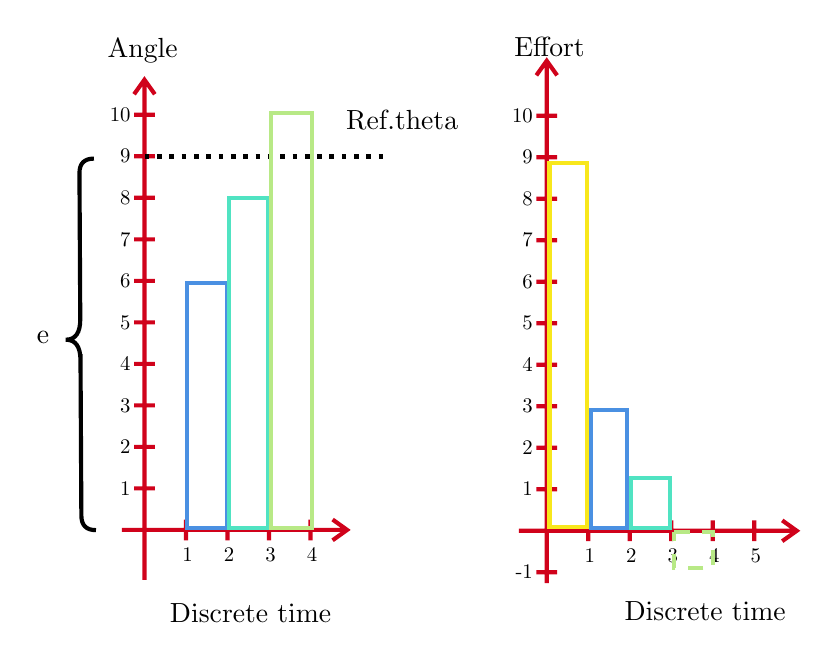
\begin{tikzpicture}[x=0.75pt,y=0.75pt,yscale=-1,xscale=1]
%uncomment if require: \path (0,530); %set diagram left start at 0, and has height of 530

%Shape: Axis 2D [id:dp45682595351826527] 
\draw [color={rgb, 255:red, 208; green, 2; blue, 27 }  ,draw opacity=1 ][line width=1.5]  (90,242.9) -- (198.5,242.9)(100.85,26) -- (100.85,267) (191.5,237.9) -- (198.5,242.9) -- (191.5,247.9) (95.85,33) -- (100.85,26) -- (105.85,33) (120.85,237.9) -- (120.85,247.9)(140.85,237.9) -- (140.85,247.9)(160.85,237.9) -- (160.85,247.9)(180.85,237.9) -- (180.85,247.9)(95.85,222.9) -- (105.85,222.9)(95.85,202.9) -- (105.85,202.9)(95.85,182.9) -- (105.85,182.9)(95.85,162.9) -- (105.85,162.9)(95.85,142.9) -- (105.85,142.9)(95.85,122.9) -- (105.85,122.9)(95.85,102.9) -- (105.85,102.9)(95.85,82.9) -- (105.85,82.9)(95.85,62.9) -- (105.85,62.9)(95.85,42.9) -- (105.85,42.9) ;
\draw   (127.85,254.9) node[anchor=east, scale=0.75]{1} (147.85,254.9) node[anchor=east, scale=0.75]{2} (167.85,254.9) node[anchor=east, scale=0.75]{3} (187.85,254.9) node[anchor=east, scale=0.75]{4} (97.85,222.9) node[anchor=east, scale=0.75]{1} (97.85,202.9) node[anchor=east, scale=0.75]{2} (97.85,182.9) node[anchor=east, scale=0.75]{3} (97.85,162.9) node[anchor=east, scale=0.75]{4} (97.85,142.9) node[anchor=east, scale=0.75]{5} (97.85,122.9) node[anchor=east, scale=0.75]{6} (97.85,102.9) node[anchor=east, scale=0.75]{7} (97.85,82.9) node[anchor=east, scale=0.75]{8} (97.85,62.9) node[anchor=east, scale=0.75]{9} (97.85,42.9) node[anchor=east, scale=0.75]{10} ;
%Straight Lines [id:da07124731425948538] 
\draw [line width=1.5]  [dash pattern={on 1.69pt off 2.76pt}]  (101,63) -- (218.5,63) ;


%Shape: Brace [id:dp5273011604952158] 
\draw  [line width=1.5]  (76.5,64) .. controls (71.83,64.03) and (69.51,66.37) .. (69.54,71.04) -- (69.93,141.23) .. controls (69.97,147.9) and (67.66,151.24) .. (62.99,151.27) .. controls (67.66,151.24) and (70.01,154.56) .. (70.04,161.23)(70.03,158.23) -- (70.46,236.04) .. controls (70.49,240.71) and (72.83,243.03) .. (77.5,243) ;
%Shape: Rectangle [id:dp5387283033097741] 
\draw  [color={rgb, 255:red, 74; green, 144; blue, 226 }  ,draw opacity=1 ][line width=1.5]  (121.5,124) -- (140.5,124) -- (140.5,242) -- (121.5,242) -- cycle ;
%Shape: Rectangle [id:dp6947960238766453] 
\draw  [color={rgb, 255:red, 80; green, 227; blue, 194 }  ,draw opacity=1 ][line width=1.5]  (141.67,83) -- (160.5,83) -- (160.5,242) -- (141.67,242) -- cycle ;
%Shape: Rectangle [id:dp8600292583953892] 
\draw  [color={rgb, 255:red, 184; green, 233; blue, 134 }  ,draw opacity=1 ][line width=1.5]  (161.67,42) -- (181.67,42) -- (181.67,242) -- (161.67,242) -- cycle ;
%Shape: Axis 2D [id:dp2561048365476184] 
\draw [color={rgb, 255:red, 208; green, 2; blue, 27 }  ,draw opacity=1 ][line width=1.5]  (281.28,243.33) -- (415.13,243.33)(294.67,16.89) -- (294.67,268.49) (408.13,238.33) -- (415.13,243.33) -- (408.13,248.33) (289.67,23.89) -- (294.67,16.89) -- (299.67,23.89) (314.67,238.33) -- (314.67,248.33)(334.67,238.33) -- (334.67,248.33)(354.67,238.33) -- (354.67,248.33)(374.67,238.33) -- (374.67,248.33)(394.67,238.33) -- (394.67,248.33)(289.67,223.33) -- (299.67,223.33)(289.67,203.33) -- (299.67,203.33)(289.67,183.33) -- (299.67,183.33)(289.67,163.33) -- (299.67,163.33)(289.67,143.33) -- (299.67,143.33)(289.67,123.33) -- (299.67,123.33)(289.67,103.33) -- (299.67,103.33)(289.67,83.33) -- (299.67,83.33)(289.67,63.33) -- (299.67,63.33)(289.67,43.33) -- (299.67,43.33)(289.67,263.33) -- (299.67,263.33) ;
\draw   (321.67,255.33) node[anchor=east, scale=0.75]{1} (341.67,255.33) node[anchor=east, scale=0.75]{2} (361.67,255.33) node[anchor=east, scale=0.75]{3} (381.67,255.33) node[anchor=east, scale=0.75]{4} (401.67,255.33) node[anchor=east, scale=0.75]{5} (291.67,223.33) node[anchor=east, scale=0.75]{1} (291.67,203.33) node[anchor=east, scale=0.75]{2} (291.67,183.33) node[anchor=east, scale=0.75]{3} (291.67,163.33) node[anchor=east, scale=0.75]{4} (291.67,143.33) node[anchor=east, scale=0.75]{5} (291.67,123.33) node[anchor=east, scale=0.75]{6} (291.67,103.33) node[anchor=east, scale=0.75]{7} (291.67,83.33) node[anchor=east, scale=0.75]{8} (291.67,63.33) node[anchor=east, scale=0.75]{9} (291.67,43.33) node[anchor=east, scale=0.75]{10} (291.67,263.33) node[anchor=east, scale=0.75]{-1} ;
%Shape: Rectangle [id:dp9341644709395209] 
\draw  [color={rgb, 255:red, 248; green, 231; blue, 28 }  ,draw opacity=1 ][line width=1.5]  (296,66) -- (314,66) -- (314,241.33) -- (296,241.33) -- cycle ;
%Shape: Rectangle [id:dp4499585049078272] 
\draw  [color={rgb, 255:red, 74; green, 144; blue, 226 }  ,draw opacity=1 ][line width=1.5]  (315.83,185) -- (333.33,185) -- (333.33,242) -- (315.83,242) -- cycle ;
%Shape: Rectangle [id:dp5245979736475872] 
\draw  [color={rgb, 255:red, 80; green, 227; blue, 194 }  ,draw opacity=1 ][line width=1.5]  (335.33,218) -- (354,218) -- (354,242) -- (335.33,242) -- cycle ;
%Shape: Rectangle [id:dp4864189057319952] 
\draw  [color={rgb, 255:red, 184; green, 233; blue, 134 }  ,draw opacity=1 ][dash pattern={on 5.63pt off 4.5pt}][line width=1.5]  (356,244) -- (374.67,244) -- (374.67,261.33) -- (356,261.33) -- cycle ;

% Text Node
\draw (225,45.33) node  [align=left] {Ref.theta};
% Text Node
\draw (52,150) node  [align=left] {e};
% Text Node
\draw (100,12) node  [align=left] {Angle};
% Text Node
\draw (152,283) node  [align=left] {Discrete time};
% Text Node
\draw (296,10) node  [align=left] {Effort};
% Text Node
\draw (371,282) node  [align=left] {Discrete time};


\end{tikzpicture}
